\documentclass{article}
\usepackage{amsmath}
\usepackage{amssymb}
\usepackage{graphicx}
\usepackage{hyperref}
\usepackage[version=4]{mhchem}


\begin{document}
\(A B\) is the diameter and \(E F\) is the chord of circle \(O . A B=10, E F=\) 6. \(A C\) and \(B D\) are the distances from \(A, B\) to chord \(E F\), respectively. Find the value of \(A C+B D\).

Solution: 8.\\
Connect \(O E\). Take \(M\), the midpoint of \(M N\). Connect \(O M\).\\
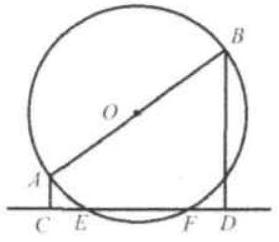
\includegraphics[width=\textwidth]{images/152(3).jpg} \(O M \perp E F\). In \(\triangle O M E, O E=\frac{1}{2} A B=5\).\\
\(E M=\frac{1}{2} E F=3\).\\
\(O M=\sqrt{O E^{2}-E M^{2}}=\sqrt{5^{2}-3^{2}}=4\).\\
\centering
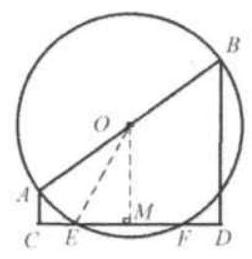
\includegraphics[width=\textwidth]{images/152(2).jpg}

So \(O M\) is the median of trapezoid \(A C D B\). Thus \(A C+B D=2 O M=2 \times 4=8\).\\

\end{document}
